\section{Results}
\subsection{Low Noise Amplifier}
Fig. ~\ref{fig:s11} shows the S11 parameters of the LNA, which indicates the input matching quality. The minimum input matching is -21 dB. Fig. ~\ref{fig:s22}, the S22, output matching is presented. The minimum matching point is -33 dB. Also, the gain (S21 parameters) can be seen from Fig. ~\ref{fig:s21}. This LNA provides a relative high gain, 17.5 dB. To show the linearity property of the LNA, the 1 dB compression point plot is presented in Fig. ~\ref{fig:lna1db}. From the figure, the 1 dB compression point is -16.46 dBm. Also, the IIP3 is preformed in cadence simulation, which is shown in Fig. ~\ref{fig:lnaiip3}. The IIP3 point is -7.77 dBm. Noise Figure and minimum Noise Figure of the LNA is presented In Fig. ~\ref{fig:lnanoise} and Fig. ~\ref{fig:lnanoisemin} respectively. The Noise Figure is 3.4 dB and the minimum Noise Figure is 1.2 dB. To match the design requirement, the DC power consumption of the LNA is 0.57 mW. 

%s11
\begin{figure}[h]
   \centering
    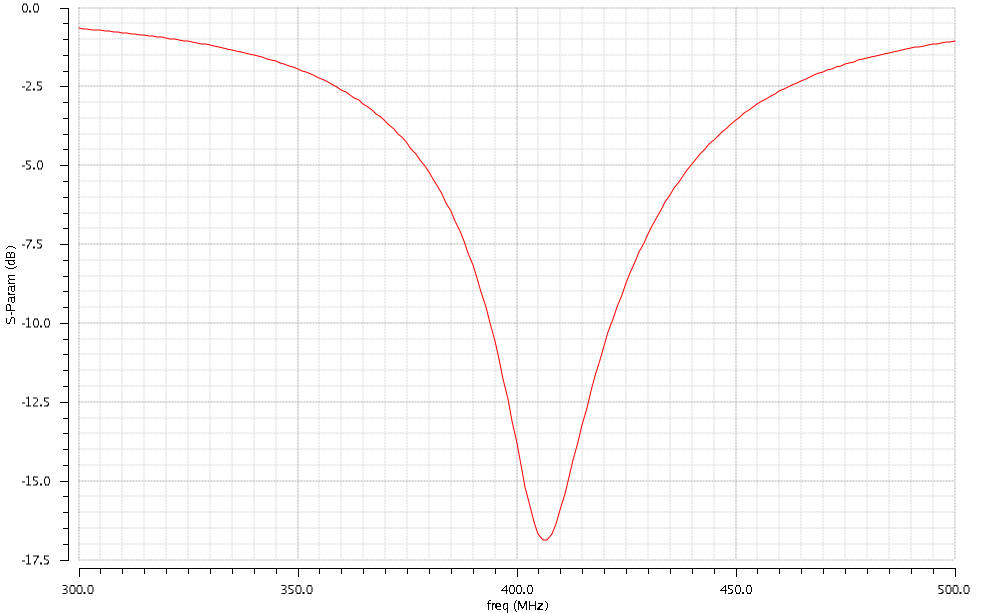
\includegraphics[width=0.5\textwidth]{figures/s11.png}
    \caption{Graph of LNA S11 input matching}
    \label{fig:s11}
\end{figure}

%s22
\begin{figure}[h]
   \centering
    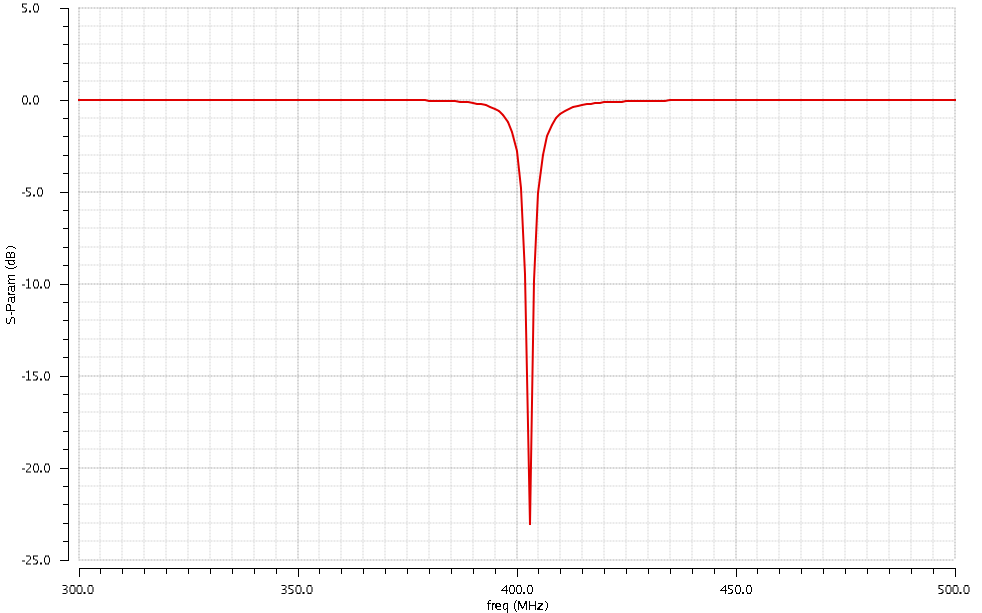
\includegraphics[width=0.5\textwidth]{figures/s22.png}
    \caption{Graph of LNA S22 output matching}
    \label{fig:s22}
\end{figure}

%s21
\begin{figure}[h]
   \centering
    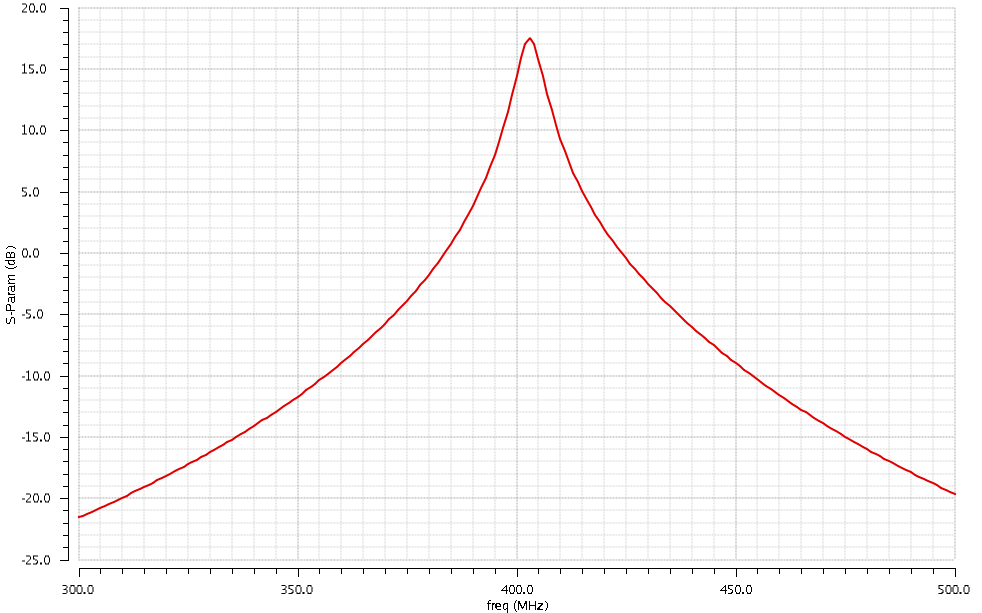
\includegraphics[width=0.5\textwidth]{figures/s21.png}
    \caption{Graph of LNA S21 gain}
    \label{fig:s21}
\end{figure}

%1dbcompression
\begin{figure}[h]
   \centering
    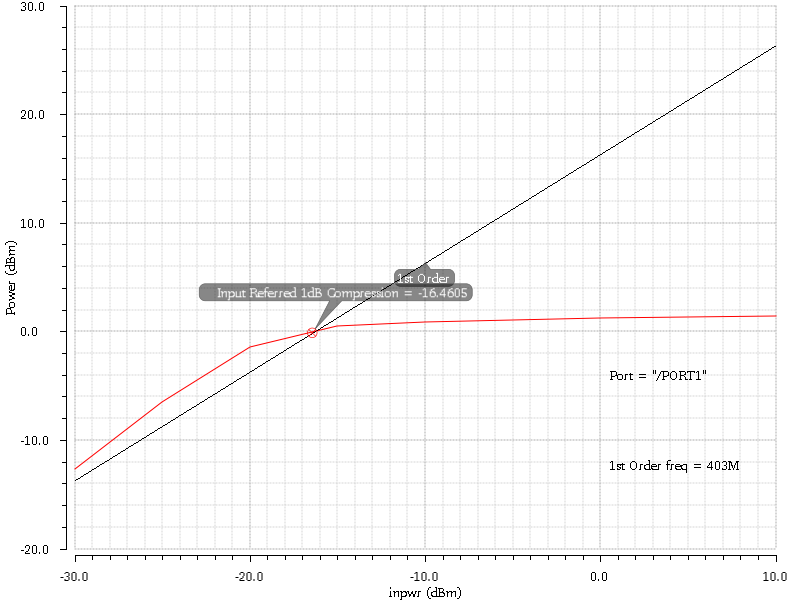
\includegraphics[width=0.5\textwidth]{figures/lna1db.png}
    \caption{LNA 1 dB compression point}
    \label{fig:1db}
\end{figure}

%IIP3
\begin{figure}[h]
   \centering
    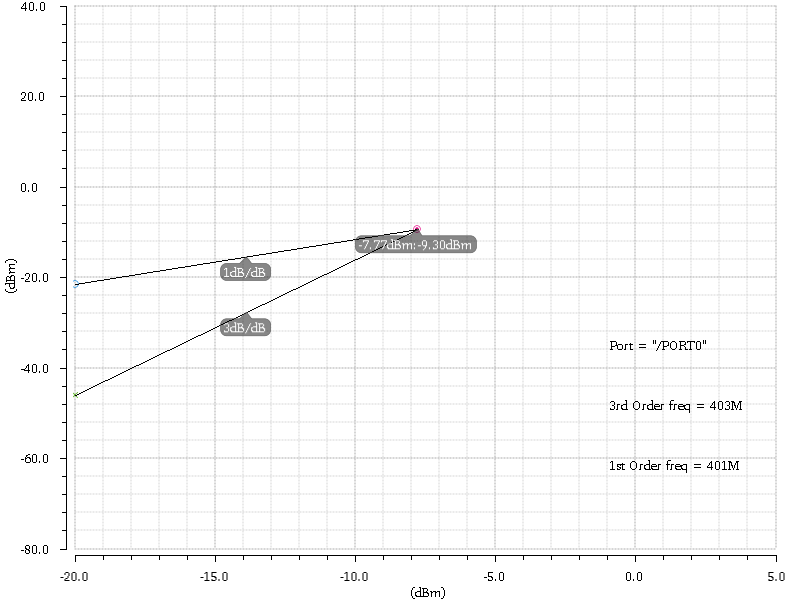
\includegraphics[width=0.5\textwidth]{figures/lnaiip3.png}
    \caption{LNA Linearity}
    \label{fig:lnaiip3}
\end{figure}

%noise
\begin{figure}[h]
   \centering
    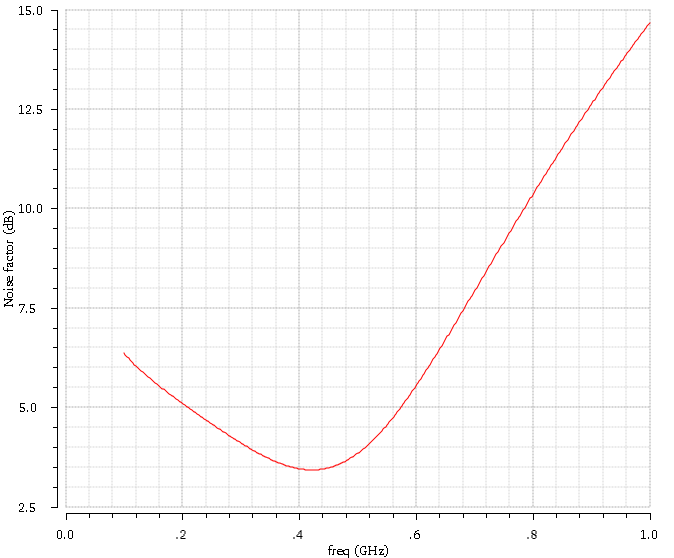
\includegraphics[width=0.5\textwidth]{figures/lnanoise.png}
    \caption{Graph of LNA noise figure}
    \label{fig:lnanoise}
\end{figure}

%min noise
\begin{figure}[h]
   \centering
    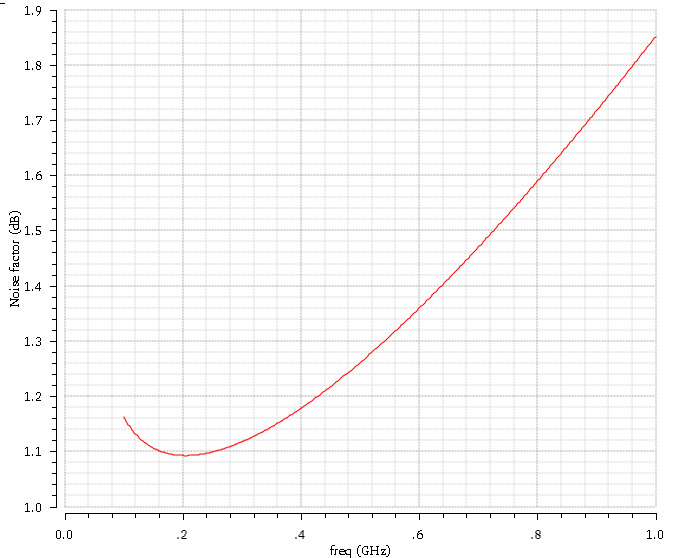
\includegraphics[width=0.5\textwidth]{figures/lnanoisemin.png}
    \caption{Graph of LNA minimum noise figure}
    \label{fig:lnanoisemin}
\end{figure}

\subsection{Mixer}
Although the assignment only asked to see conversion gain with respect to frequency as shown in Fig. ~\ref{fig:cgfreq} we also simulated for conversion gain with respect to input power as shown in Fig. ~\ref{fig:cgpwr}. These graphs show that the mixer is able to maintain good gain across the frequencies of interest as well as consistent gain across sensitivities as low as -100 dBm. Fig. ~\ref{fig:loif} and Fig. ~\ref{fig:lorf} show the VCO feedthrough to the input and output ports. As can be seen in the graphs, the setup of the mixer causes these figures to be very low. The noise of the mixer was found to be 4.40 dB as shown in Fig. ~\ref{fig:mixernoise}. Lastly, the linearity of the mixer can be found in Fig. ~\ref{fig:mixerlin}. The linearity is quite lower than expected however this was a trade-off to achieve a high gain and low noise. Final mixer results can be found in TABLE ~\ref{tab:mixerresults}.

%table of results
\begin{table}[h]
\begin{center}
	\begin{tabular}{ |c | c | }
 		\hline                      
  		Conversion gain &  10.50 dB\\ \hline
  		LO-IF feedthrough &  -75.06 dB\\ \hline
  		LO-RF feedthrough & -103.40 dB\\ \hline
		Noise Figure &  4.40 dB\\ \hline
		IIP3 & -13.26 dBm\\ \hline
		Power & 0.8 mW \\ 
  		\hline  
	\end{tabular}

\end{center}
\caption{Final results from Mixer simulations}
\label{tab:mixerresults}
\end{table}

%mixer conversion gain vs frequency
\begin{figure}[h]
   \centering
    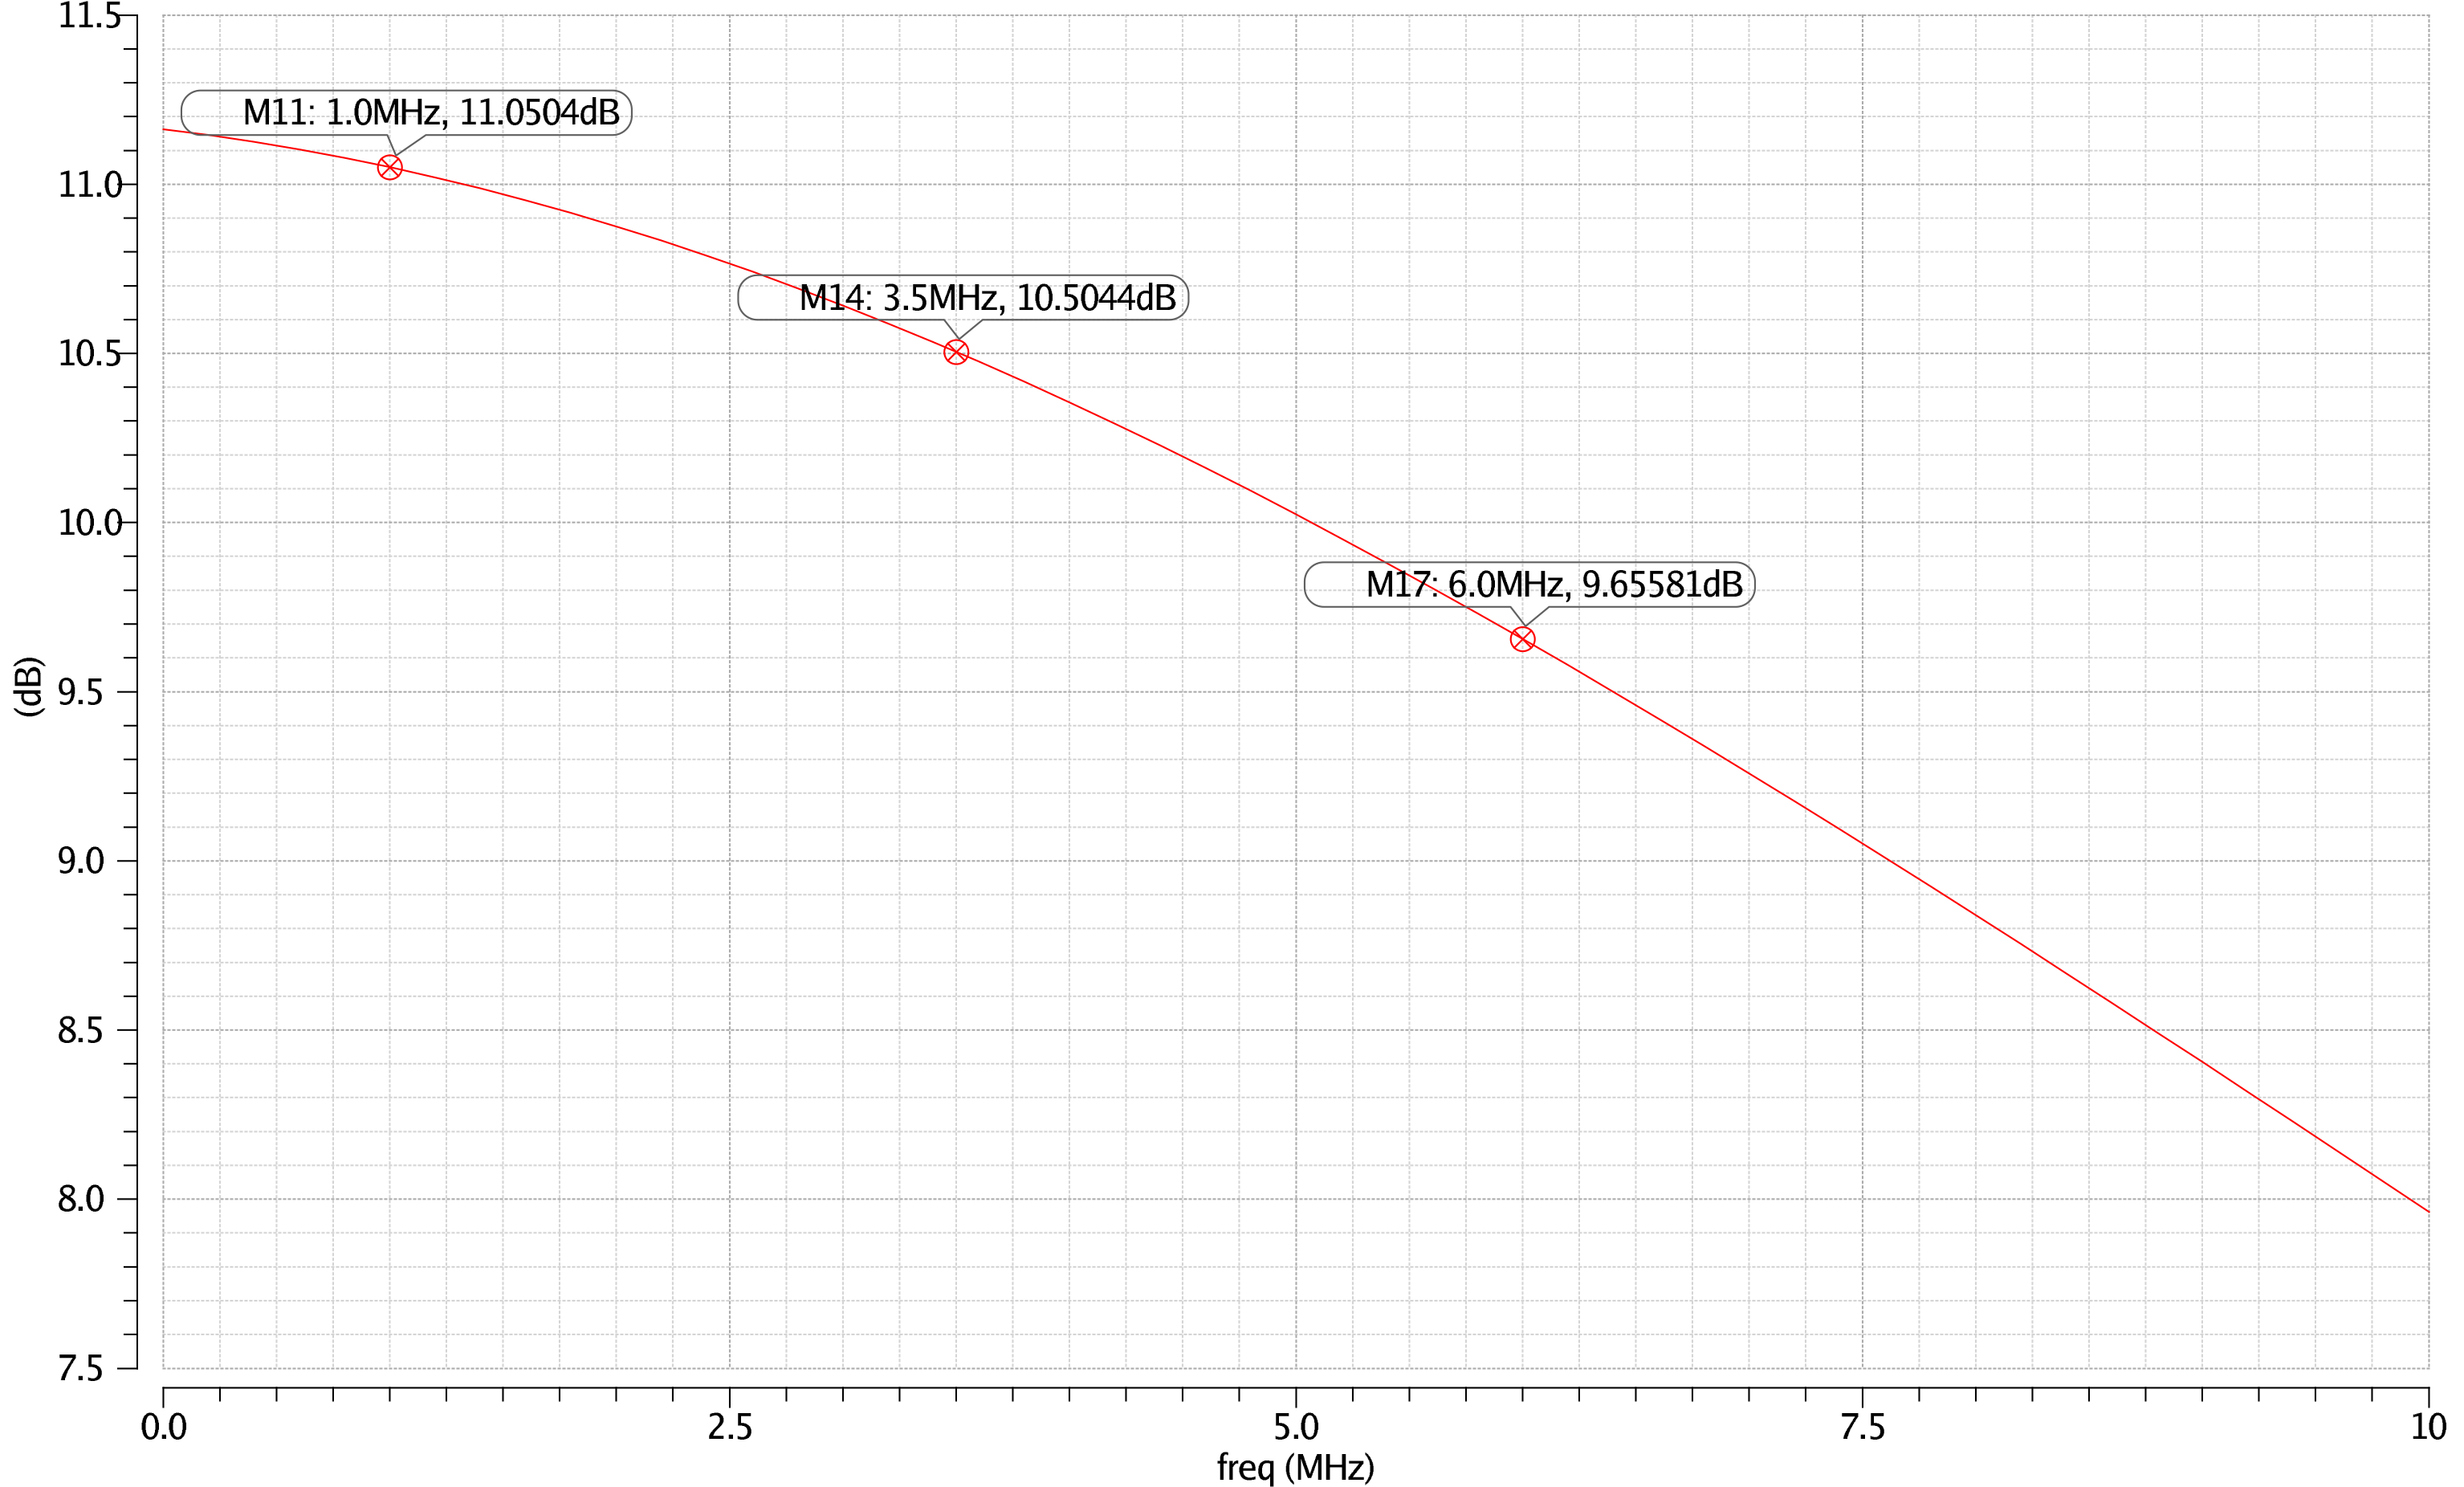
\includegraphics[width=0.5\textwidth]{figures/MixerConversionGainFreq.png}
    \caption{Mixer conversion gain with respect to frequency}
    \label{fig:cgfreq}
\end{figure}

%mixer conversion gain vs power
\begin{figure}[h]
   \centering
    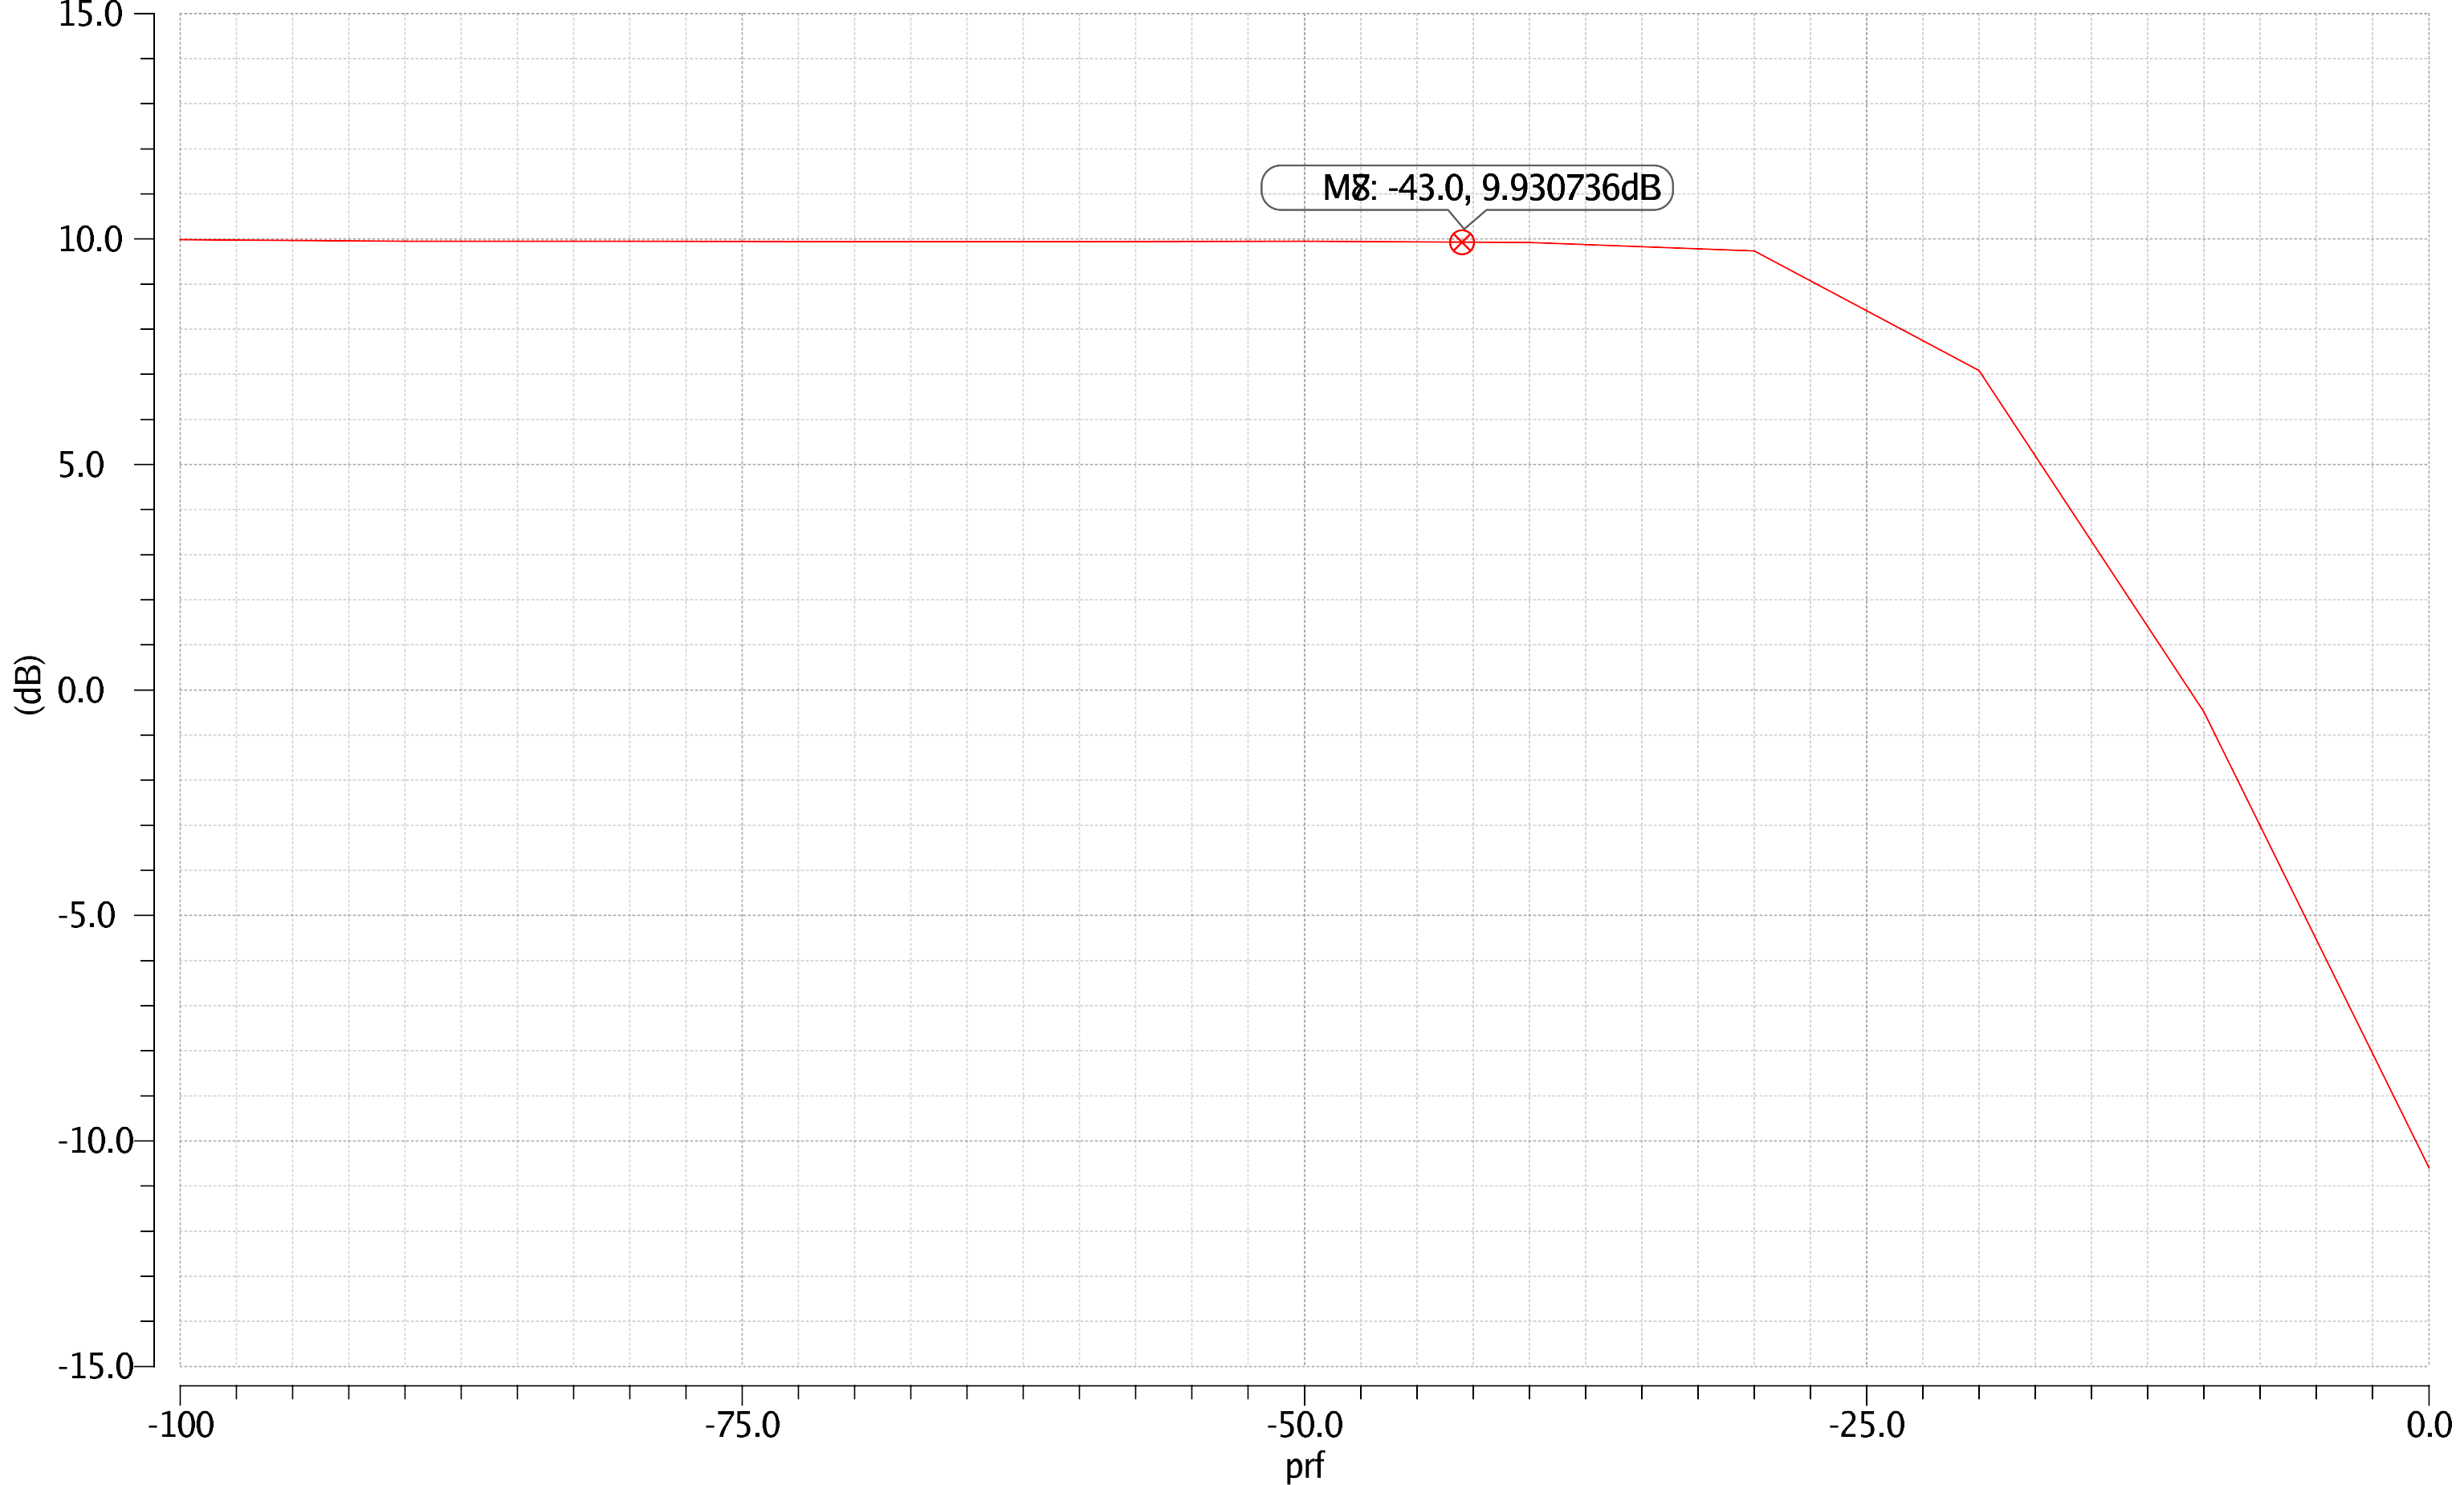
\includegraphics[width=0.5\textwidth]{figures/MixerConversionGain.png}
    \caption{Mixer conversion gain with respect to input power}
    \label{fig:cgpwr}
\end{figure}


%LO-IF feedthrough
\begin{figure}[h]
   \centering
    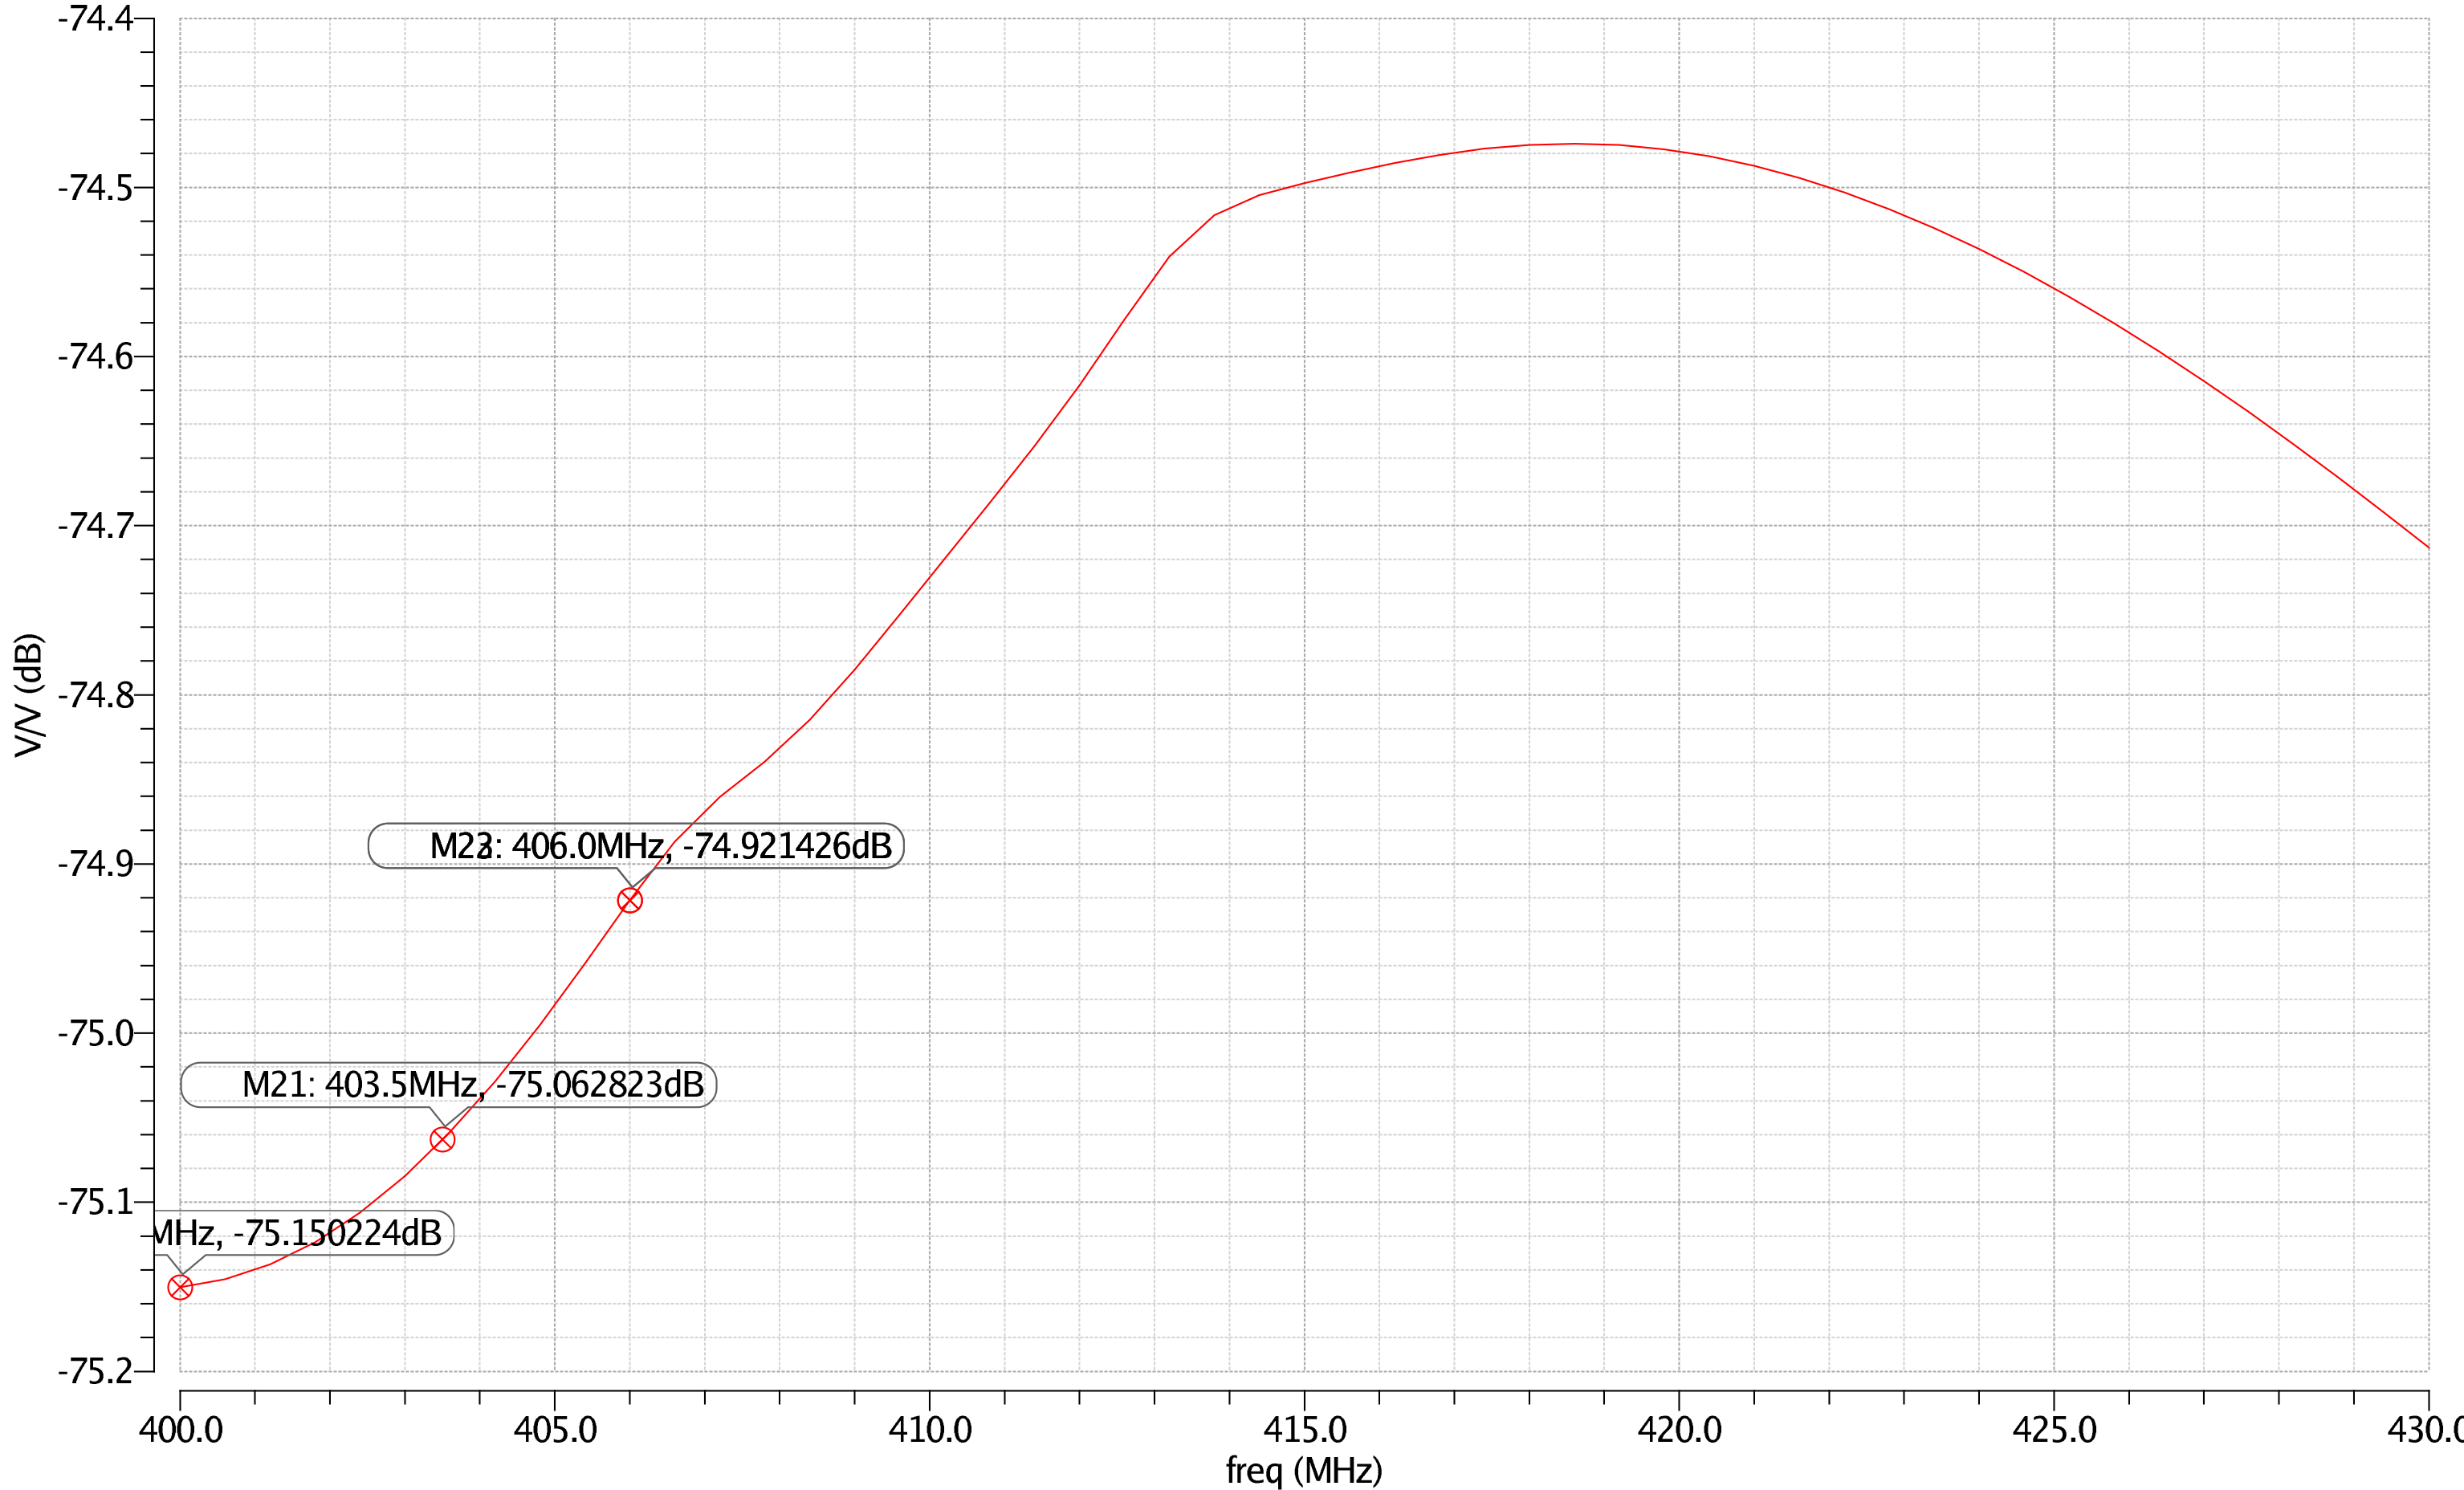
\includegraphics[width=0.5\textwidth]{figures/MixerLO-IFfeed.png}
    \caption{Mixer oscillator to IF output feedthrough}
    \label{fig:loif}
\end{figure}

%LO-RF feedthrough
\begin{figure}[h]
   \centering
    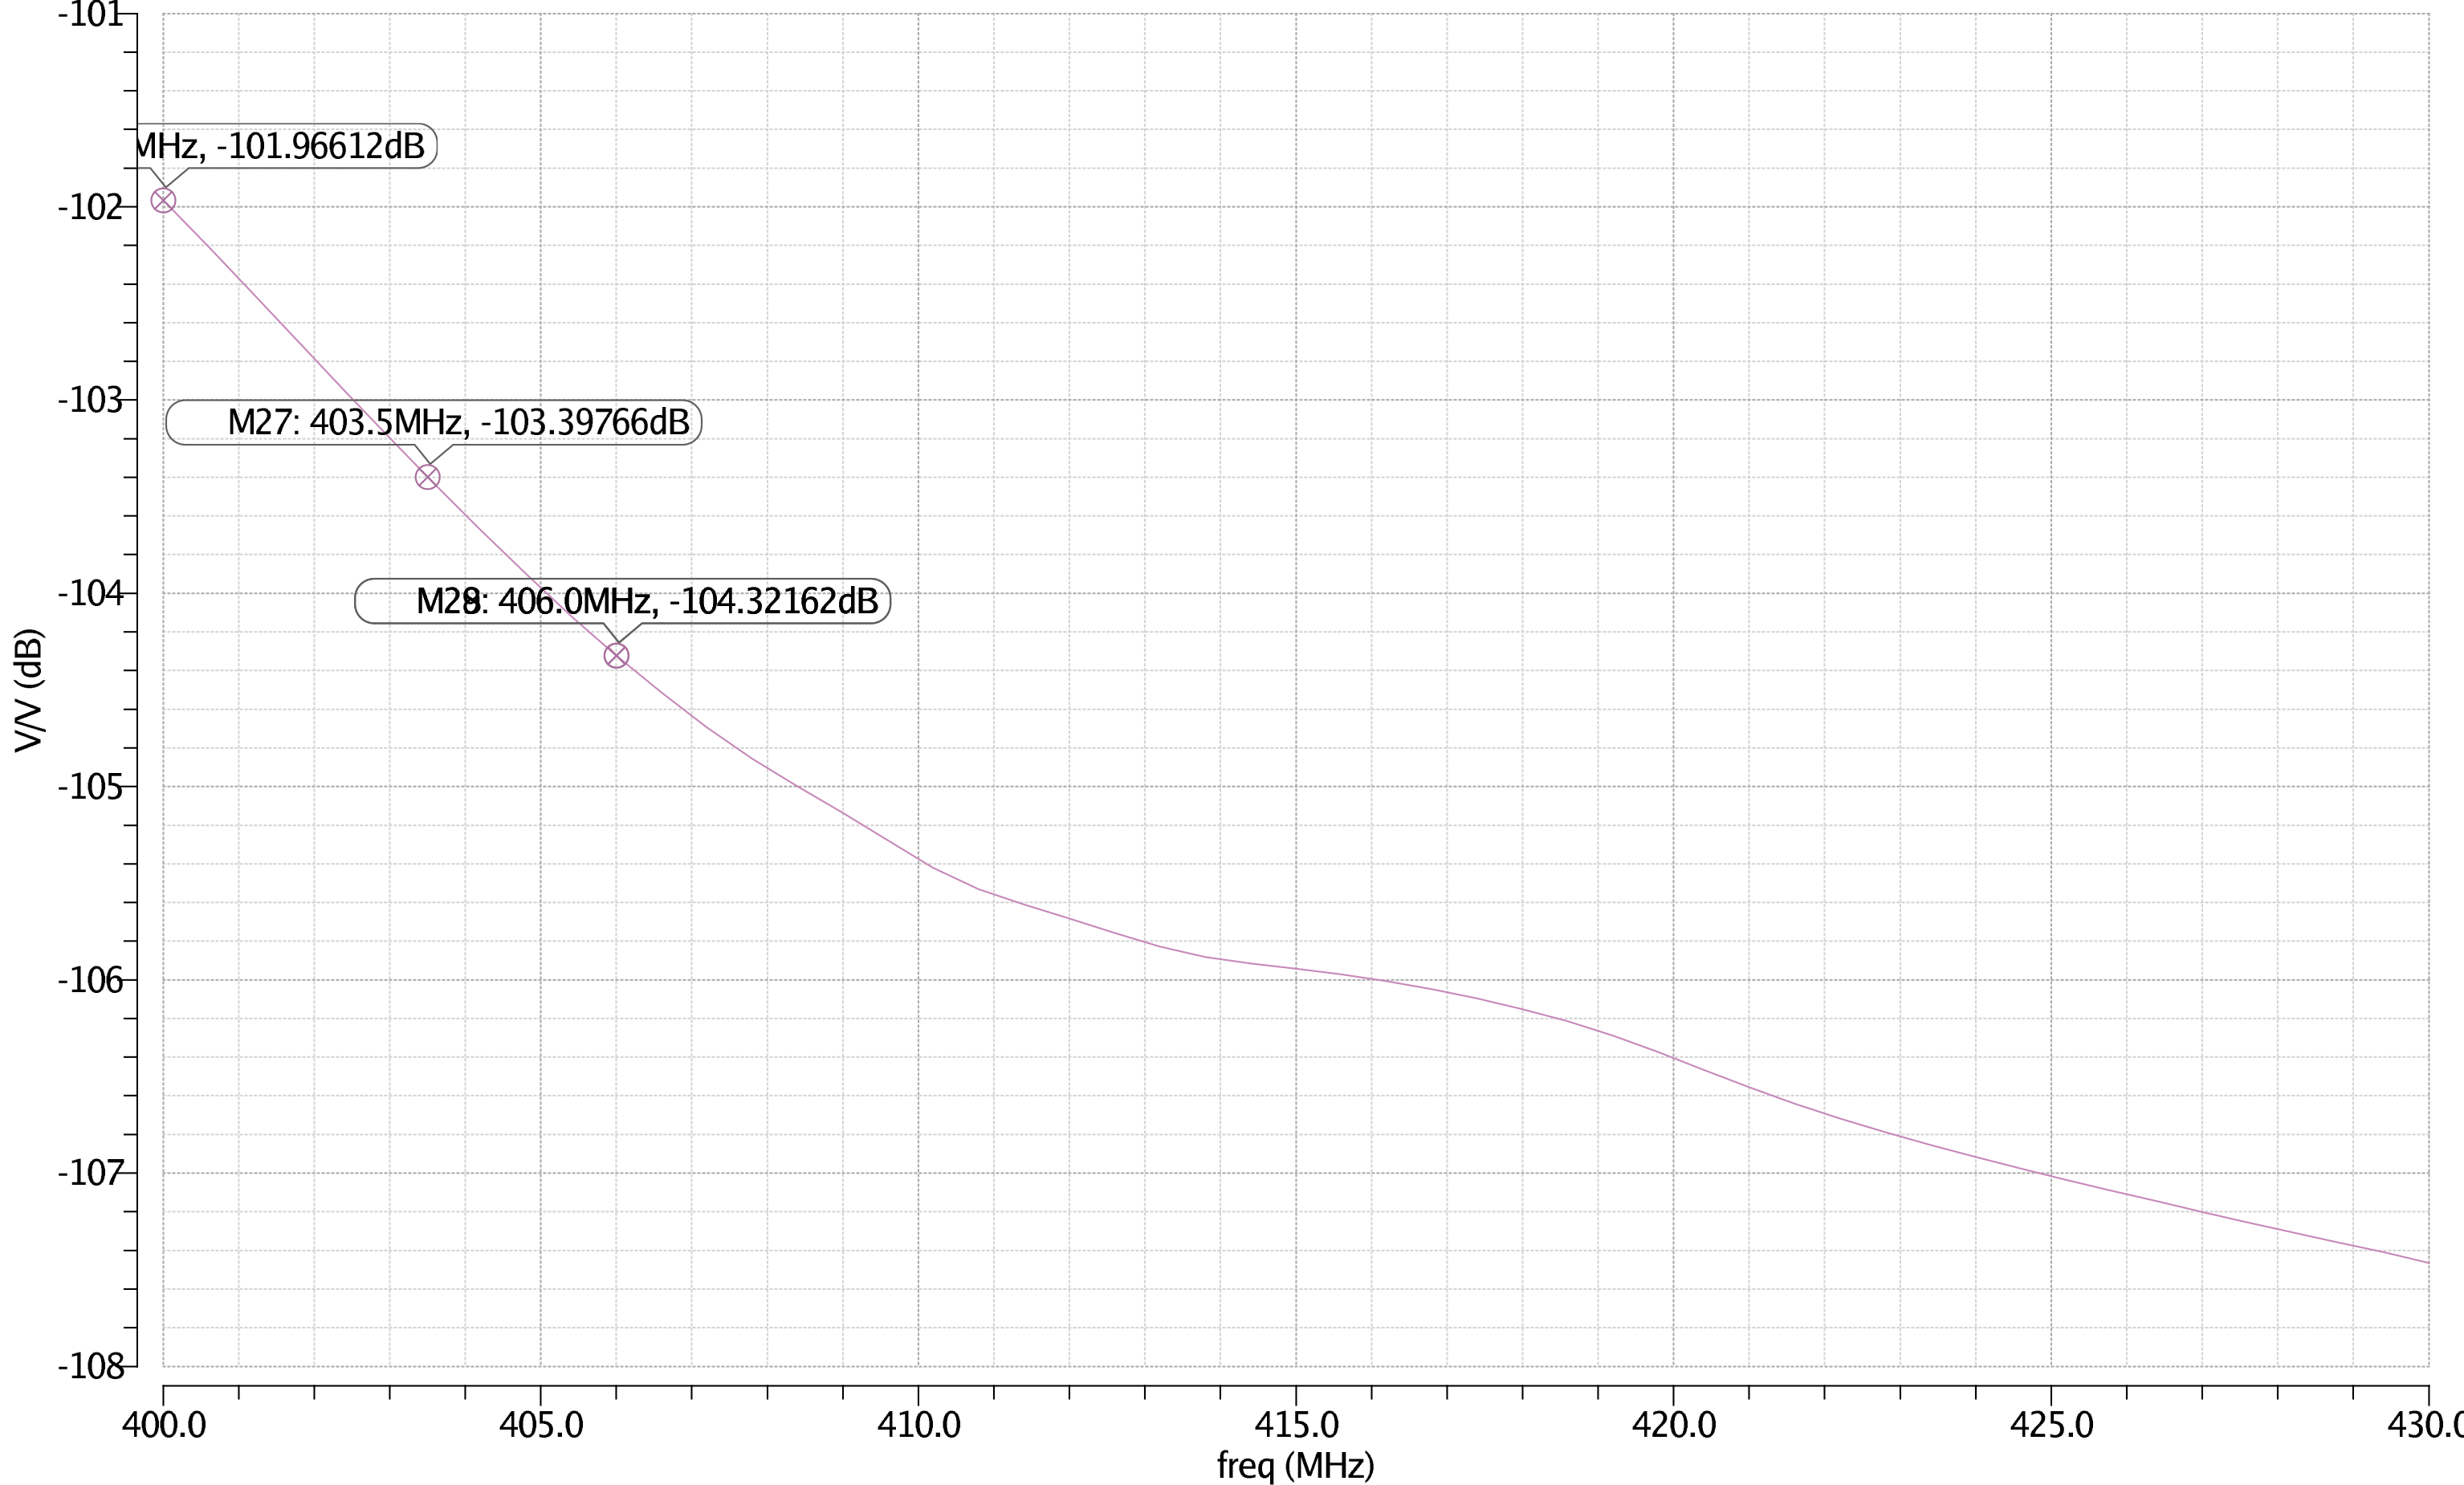
\includegraphics[width=0.5\textwidth]{figures/MixerLO-RFfeed.png}
    \caption{Mixer oscillator to RF input feedthrough}
    \label{fig:lorf}
\end{figure}

%Noise figure
\begin{figure}[h]
   \centering
    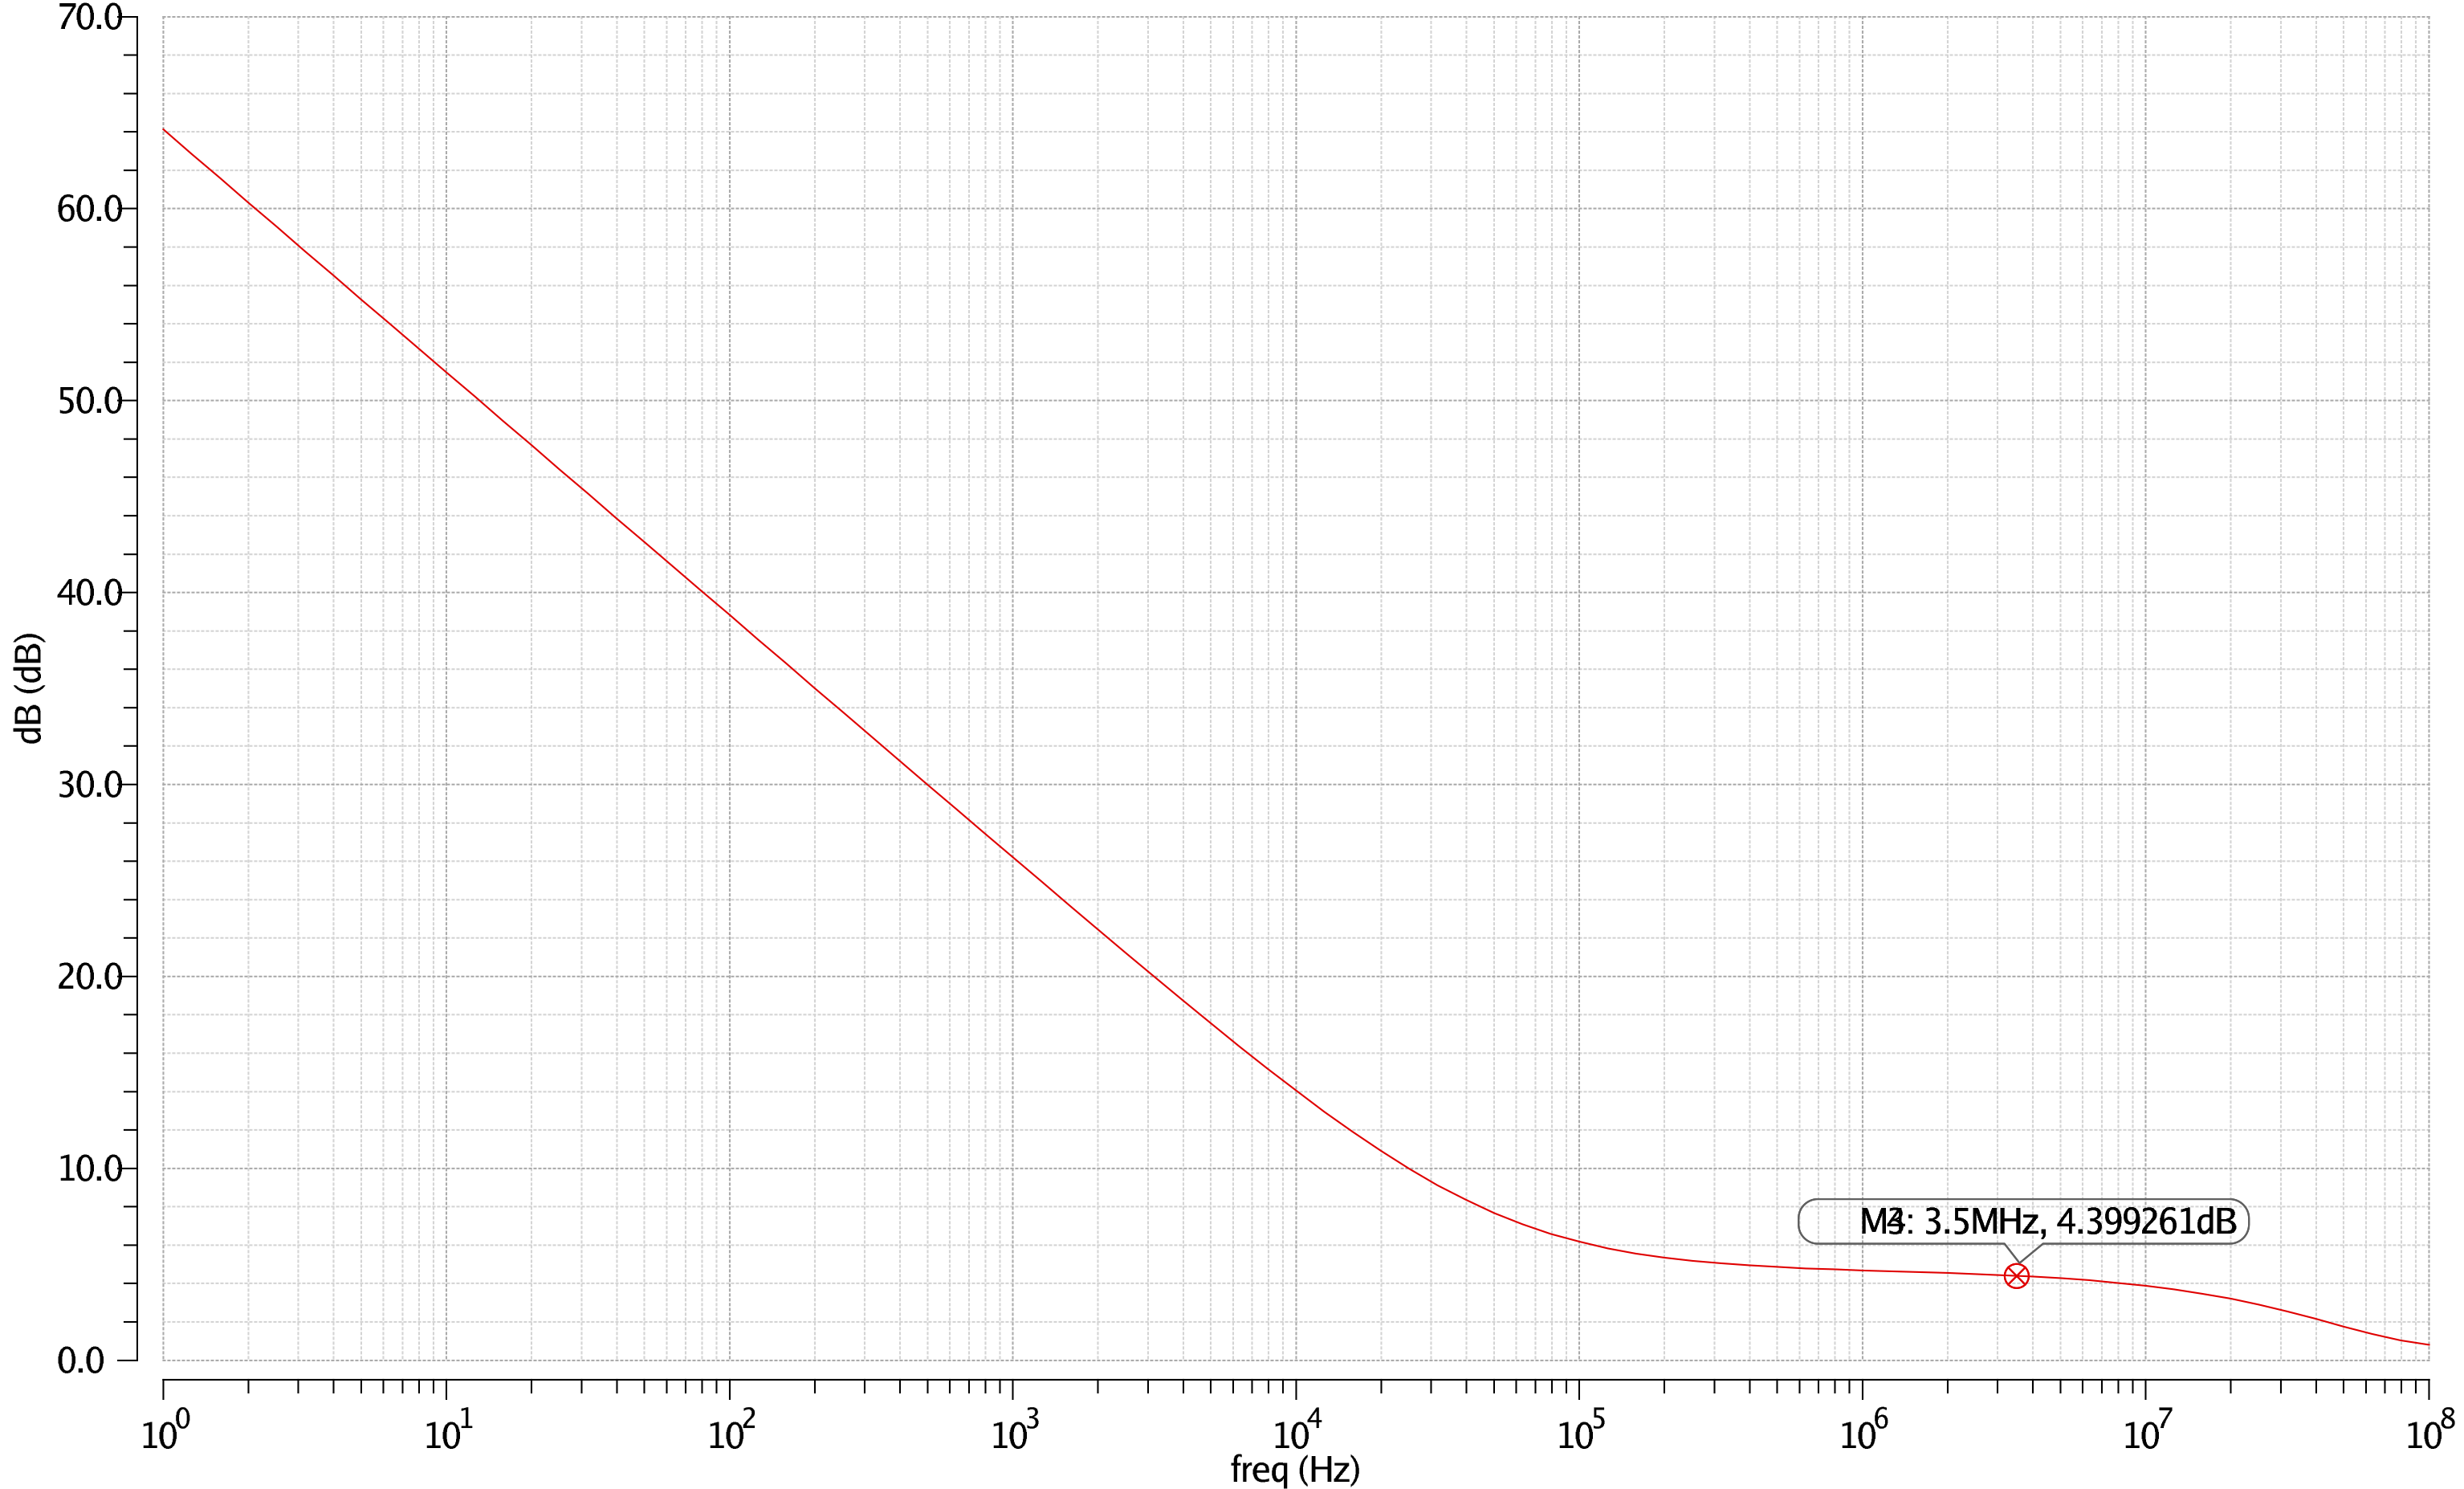
\includegraphics[width=0.5\textwidth]{figures/MixerNoiseFigure.png}
    \caption{Graph of Mixer Noise Figure}
    \label{fig:mixernoise}
\end{figure}

%Linearity
\begin{figure}[h]
   \centering
    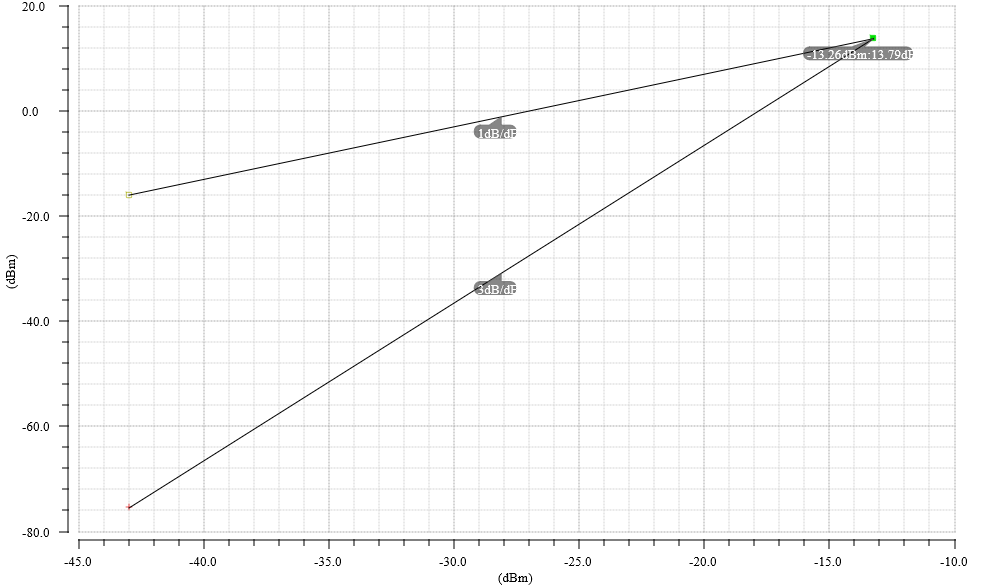
\includegraphics[width=0.5\textwidth]{figures/mixerIIP3.png}
    \caption{Graph of Mixer linearity}
    \label{fig:mixerlin}
\end{figure}

\subsection{Voltage Controlled Oscillator}
Fig.~\ref{fig:vcotrans} shows the simulated output transients of the proposed VCO; the VCO provides two differential outputs with the same peak-peak value of 305 mV. The oscillation frequency can also be calculated from the period of sinusoidal waveform, which is 400 MHz. The phase noise is shown in Fig. ~\ref{fig:vcophase} and it is -119 $\frac{dBc}{Hz}$ at 1 MHz offset from the center frequency of 400 MHz. Fig. ~\ref{fig:vcotune} plots the simulated tuning curve by varying the controllable voltage. As the tuning voltage sweeps from -0.5 V to 1 V, the oscillation frequency changes from 393 MHz to 400 MHz, indicating a tunable range of 6 MHz. The VCO’s power consumption, which is a critical consideration in MedRadio application, is 0.2 mW. A table of results can be found in TABLE ~\ref{tab:vcoresults}.

%table of results
\begin{table}[h]
\begin{center}
	\begin{tabular}{ |c | c | }
 		\hline                      
  		Tuning Range &  6 MHz \\ \hline
  		Phase noise &  -119 $\frac{dBc}{Hz}$ \\ \hline
		Power & 0.2 mW \\ 
  		\hline  
	\end{tabular}

\end{center}
\caption{Final results from VCO simulations}
\label{tab:vcoresults}
\end{table}

%VCO Trans
\begin{figure}[h]
   \centering
    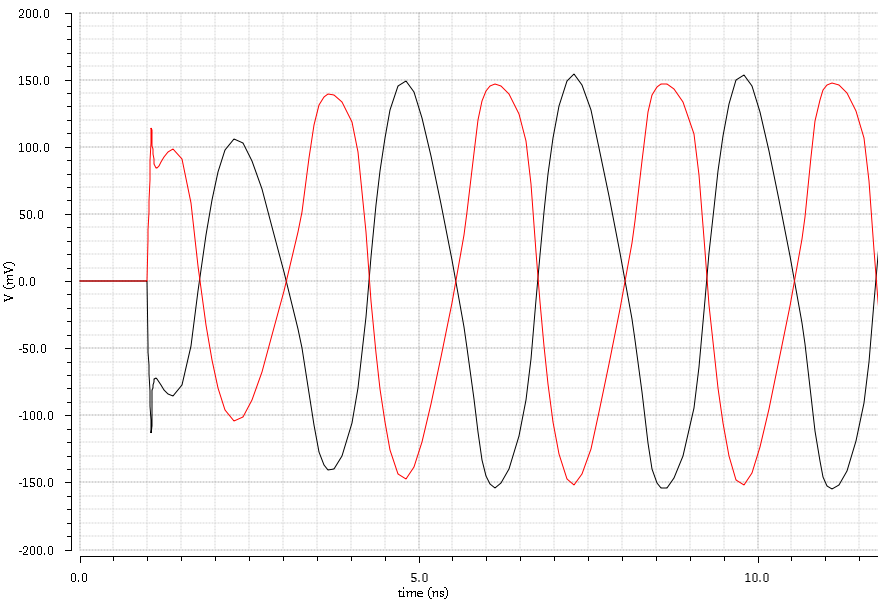
\includegraphics[width=0.5\textwidth]{figures/VCOTrans.png}
    \caption{Graph of VCO transient response}
    \label{fig:vcotrans}
\end{figure}

%VCO Phase Noise
\begin{figure}[h]
   \centering
    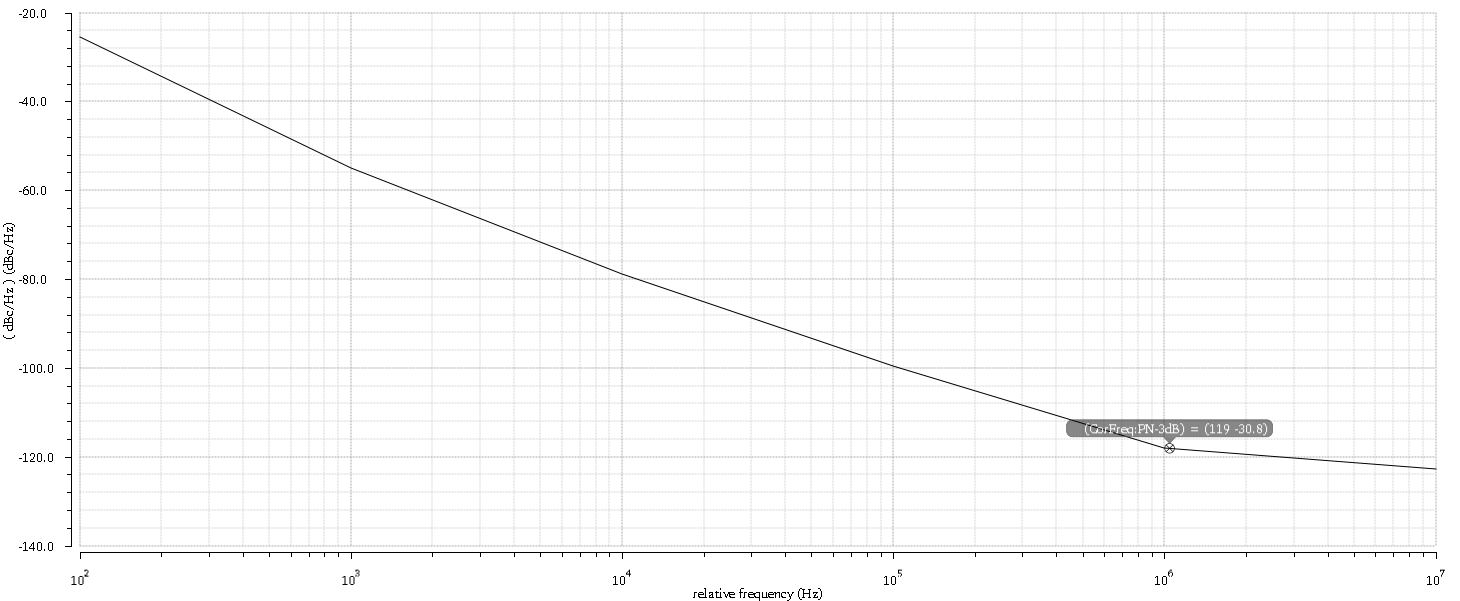
\includegraphics[width=0.5\textwidth]{figures/VCOPhaseNoise.png}
    \caption{Graph of VCO phase noise}
    \label{fig:vcophase}
\end{figure}

%Tunning curve
\begin{figure}[h]
   \centering
    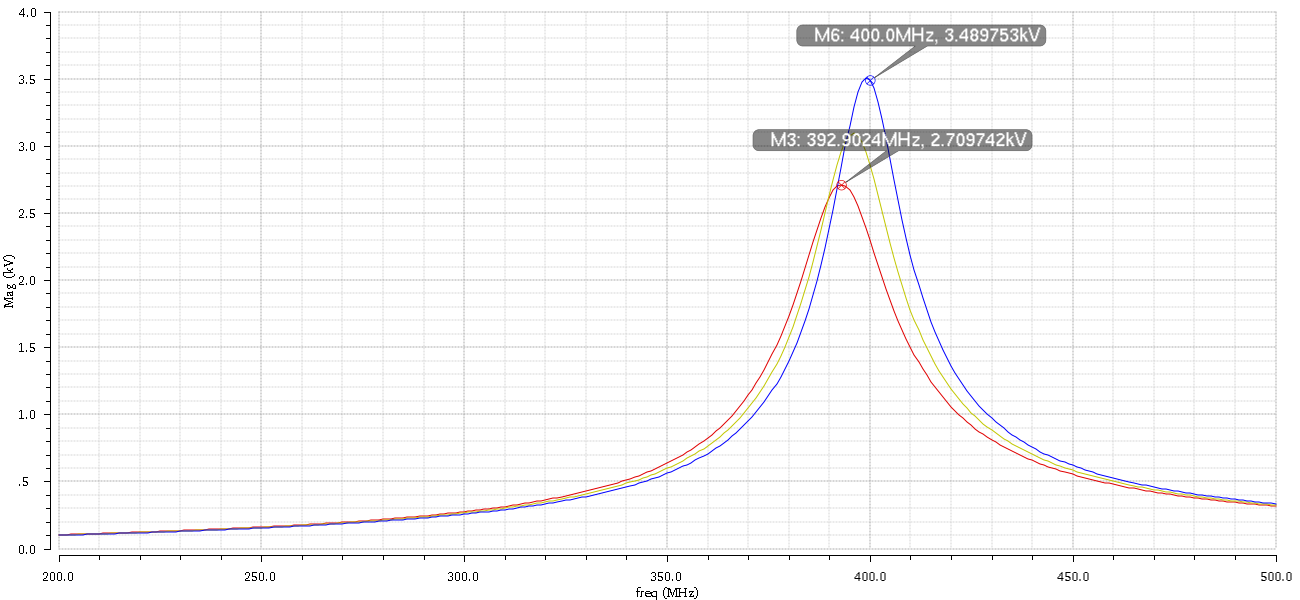
\includegraphics[width=0.5\textwidth]{figures/VCOTuning.png}
    \caption{Graph of VCO tuning curve}
    \label{fig:vcotune}
\end{figure}